\chapter{Démarche de projet}

\section{Méthodologie adoptée }

Dans le cadre du développement de l’application mobile URGmetEO, une méthodologie de travail structurée a été adoptée afin d’assurer une progression cohérente du projet, depuis l’analyse des besoins jusqu’au déploiement de la solution. Étant donné que le projet comporte plusieurs composantes, notamment l’interface mobile, le backend, l’API et l’organisation des données météorologiques, il était nécessaire d’utiliser une approche permettant de planifier les tâches, de suivre l’avancement et de faciliter les ajustements en cours de réalisation.

\noindent Le choix s’est porté sur une démarche inspirée de la méthode Agile. Cette approche est particulièrement adaptée aux projets informatiques, car elle favorise un développement progressif, itératif et collaboratif. Au lieu de concevoir tout le système d’un seul bloc, le projet est découpé en plusieurs phases de travail, chacune permettant de produire une partie fonctionnelle de l’application, puis de l’améliorer progressivement.

\noindent Dans le cas de URGmetEO, cette méthodologie a permis d’avancer par étapes, en commençant par la définition des besoins et des fonctionnalités principales, puis par la conception de l’architecture générale du système, avant de passer à l’implémentation du backend et de l’interface utilisateur. Elle a également facilité les phases de test, de correction et d’intégration des différents modules du système.

\noindent Ainsi, la méthodologie adoptée a constitué un cadre d’organisation efficace pour conduire le projet de manière progressive, tout en gardant une certaine souplesse face aux ajustements techniques et fonctionnels rencontrés pendant le développement.

\begin{figure}[H]
    \centering
   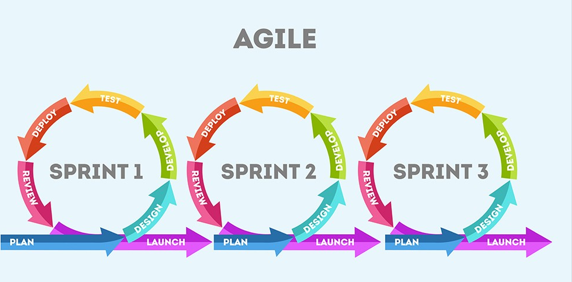
\includegraphics[width=1\textwidth]{Capture d'écran 2026-03-20 181055.png}
    \caption{La methode argile}
    \label{fig:placeholder}
\end{figure}
\newpage

\subsection{Méthode Agile – Activités d’ingénierie logicielle}

La méthodologie Agile adoptée dans le cadre du projet URGmetEO repose sur un ensemble d’activités fondamentales issues de l’ingénierie logicielle. Ces activités permettent d’organiser le développement de manière structurée tout en conservant une certaine flexibilité.

\noindent La première étape consiste en l’analyse des besoins. Elle permet d’identifier les fonctionnalités principales de l’application, telles que l’affichage des données météorologiques, la géolocalisation, les prévisions ou encore les alertes. Cette phase est essentielle pour définir les attentes des utilisateurs et orienter le développement du système.

\noindent Ensuite, une phase de conception est réalisée. Elle consiste à définir l’architecture du système ainsi que les différents composants qui le constituent, notamment le backend, l’API, la base de données et l’interface utilisateur. Cette étape inclut également la modélisation du système à l’aide d’outils comme les diagrammes UML.

\noindent La phase d’implémentation correspond au développement concret de l’application. Elle comprend la mise en place du serveur backend avec Node.js et Express, ainsi que le développement de l’interface mobile à l’aide de technologies adaptées. Cette étape est réalisée de manière progressive, en intégrant les différentes fonctionnalités au fur et à mesure.

\noindent Par la suite, des tests sont effectués afin de vérifier le bon fonctionnement des différentes parties du système. Ces tests permettent de détecter et de corriger les erreurs, d’améliorer les performances et de garantir la fiabilité de l’application.

\noindent Enfin, la phase de déploiement consiste à rendre l’application accessible aux utilisateurs. Elle inclut la mise en ligne du backend sur un serveur ainsi que la préparation de l’application pour son utilisation sur les différentes plateformes.

\noindent L’ensemble de ces activités est réalisé de manière itérative, ce qui permet d’améliorer continuellement le système tout au long du projet.


\section{Structure du projet}
Le projet URGmetEO est structuré de manière modulaire. Une structure modulaire est définie comme une approche qui consiste à décomposer un système en plusieurs modules indépendants, chacun responsable d’une fonctionnalité spécifique, tout en permettant leur interaction au sein d’un même système. Cette approche facilite le développement, la maintenance ainsi que l’évolution de l’application.

\noindent Dans ce contexte, cette organisation permet de séparer les différentes fonctionnalités du système en composants indépendants mais interconnectés.

\noindent L’architecture globale repose principalement sur une application mobile, un backend chargé du traitement des données et une base de données assurant le stockage des informations météorologiques. Cette structuration favorise une meilleure organisation du code et une intégration efficace des différentes parties du système.

\subsection{Les principaux modules}

Le système URGmetEO est composé de plusieurs modules fonctionnels et techniques, permettant d’assurer son bon fonctionnement.

\noindent \textbf{Modules fonctionnels :}

\begin{itemize}

\item \textbf{Module d’affichage météo} : affichage des conditions météorologiques en temps réel.

\item \textbf{Module de prévisions} : affichage des prévisions météorologiques sur plusieurs jours.

\item \textbf{Module de géolocalisation} : détection automatique de la position de l’utilisateur.

\item \textbf{Module de recherche} : recherche manuelle d’une ville.

\item \textbf{Module d’alertes météorologiques} : notification en cas de conditions extrêmes.

\item \textbf{Module de visualisation} : graphiques, cartes et tableaux de données.

\item \textbf{Module de configuration} : paramètres de l’application (langue, unités, thème).

\end{itemize}

\noindent \textbf{Modules techniques :}

\begin{itemize}

\item \textbf{Module backend / API} : traitement des données et communication avec le serveur.

\item \textbf{Module base de données} : stockage des informations météorologiques.

\item \textbf{Module d’authentification} : gestion des utilisateurs et sécurisation des accès (fonctionnalité évolutive).

\item \textbf{Module de gestion des erreurs} : traitement des erreurs et amélioration de la fiabilité du système.

\end{itemize}

\noindent L’ensemble de ces modules interagit afin de garantir une application performante, fiable et évolutive.


\section{Gestion du projet}

\subsection{Organisation}

Le projet URGmetEO a été réalisé en équipe, ce qui a nécessité une organisation rigoureuse afin de répartir efficacement les tâches entre les différents membres. Chaque participant a été impliqué dans plusieurs phases du projet, notamment la conception, le développement et les tests.

\noindent Dans un premier temps, les besoins du projet ont été analysés collectivement afin de définir les fonctionnalités principales du système. Par la suite, les tâches ont été réparties en fonction des compétences de chacun. Certains membres se sont principalement concentrés sur le développement du backend, tandis que d’autres ont pris en charge la partie frontend ainsi que la conception de l’interface utilisateur.

\noindent Tout au long du projet, des échanges réguliers ont permis de suivre l’avancement des travaux, de résoudre les difficultés rencontrées et d’assurer la cohérence entre les différentes composantes du système.

\subsection{Suivi avec GitHub}

Le suivi du projet a été assuré à l’aide de la plateforme GitHub, utilisée comme outil de gestion de version et de collaboration. Elle a permis de centraliser le code source, de suivre les modifications apportées et de faciliter le travail en équipe.

\noindent Chaque membre pouvait ainsi contribuer au projet en proposant des modifications à travers des commits, tout en conservant un historique des différentes versions du code. L’utilisation de GitHub a également permis de limiter les conflits de version et d’assurer une meilleure organisation du développement.

\noindent De plus, cet outil a facilité la coordination entre les membres de l’équipe, notamment grâce au partage du code et à la gestion des différentes branches du projet.

\section{Rôles et responsabilités}
\section{Déploiement}
\subsection{Serveur Web}
\subsection{Architecture générale du système}
\subsection{Déploiement sur serveur Linux / C}


\section{Sécurité}
\subsection{Sécurité du backend et des API}
\subsection{Sécurité de l'application et des données}
\subsection{Bonnes pratiques à adoptées}
\subsection{Budget prévisionnel}